% ============================================================
%  يُترجَم بـ XeLaTeX  (في Overleaf: Menu → Compiler → XeLaTeX)
%  الخط: Amiri (متوفر في Overleaf، أو حمّله من github.com/aliftype/amiri)
% ============================================================
\documentclass[12pt,a4paper]{article}
\usepackage[a4paper,margin=1.7cm,top=2.3cm,bottom=2.9cm,headheight=15pt,footskip=1.5cm]{geometry}
\usepackage{amsmath,amssymb}
\usepackage{icomma}
\usepackage[english,bidi=default,layout=lists]{babel}
\babelprovide[import,main]{arabic}
\babelfont{rm}[Scale=1.08]{Amiri}
\babelfont{sf}[Scale=1.08]{Amiri}
\usepackage[most]{tcolorbox}
\usepackage{tikz}
\usetikzlibrary{arrows.meta,calc,shadings}
\usepackage{array}
\usepackage{colortbl}
\usepackage{fancyhdr}
\usepackage{titlesec}
\usepackage{enumitem}
\usepackage{collcell}
\usepackage{needspace}
\usepackage{etoolbox}
% أعمدة جداول تُكتب خلاياها بالعربية في الاتجاه الصحيح
\newcolumntype{C}{>{\collectcell\ar}c<{\endcollectcell}}
% تجنب عنوان يتيم في أسفل الصفحة
\pretocmd{\section}{\Needspace{15\baselineskip}}{}{}
\pretocmd{\subsection}{\Needspace{11\baselineskip}}{}{}

% ---------- الألوان ----------
\definecolor{cDef}{HTML}{1F4E9C}
\definecolor{cThm}{HTML}{B3261E}
\definecolor{cRem}{HTML}{2E7D32}
\definecolor{cEx}{HTML}{C76B00}
\definecolor{cMeth}{HTML}{6A1B9A}
\definecolor{cSol}{HTML}{00695C}
\definecolor{cSec}{HTML}{1F3A68}

% ---------- العناوين ----------
\titleformat{\section}{\Large\bfseries\color{cSec}}{\thesection.}{0.6em}{}[{\color{cSec!60}\titlerule[1pt]}]
\titleformat{\subsection}{\large\bfseries\color{cThm!85!black}}{\thesubsection.}{0.5em}{}
\titlespacing*{\section}{0pt}{14pt}{8pt}
\titlespacing*{\subsection}{0pt}{10pt}{5pt}
\setlength{\parindent}{0pt}
\setlength{\parskip}{4pt}
\setlist{itemsep=2pt,topsep=3pt}

% ---------- الصناديق (تُرسم في سياق LTR ويُكتب محتواها بالعربية) ----------
\newtcolorbox{arbox}[3][]{enhanced,
  colback=#2!5,colframe=#2!80!black,arc=2mm,boxrule=0.8pt,
  left=6pt,right=6pt,top=8pt,bottom=5pt,
  fonttitle=\bfseries,coltitle=white,
  title={\foreignlanguage{arabic}{#3}},
  attach boxed title to top right={xshift=-5mm,yshift=-3mm},
  boxed title style={colback=#2!80!black,arc=1.5mm,boxrule=0pt},
  before upper={\selectlanguage{arabic}},
  before skip=8pt,after skip=8pt,breakable,#1}
\newenvironment{BOX}[2]{\begin{otherlanguage}{english}\begin{arbox}{#1}{#2}}{\end{arbox}\end{otherlanguage}}
\newenvironment{tarif}[1][تعريف]{\begin{BOX}{cDef}{#1}}{\end{BOX}}
\newenvironment{khassia}[1][خاصية]{\begin{BOX}{cThm}{#1}}{\end{BOX}}
\newenvironment{molahada}[1][ملاحظة]{\begin{BOX}{cRem}{#1}}{\end{BOX}}
\newenvironment{mithal}[1][مثال]{\begin{BOX}{cEx}{#1}}{\end{BOX}}
\newenvironment{tariqa}[1][طريقة]{\begin{BOX}{cMeth}{#1}}{\end{BOX}}

% ---------- التمارين والحلول ----------
\newcounter{exo}
\newenvironment{tamrin}[1]{\stepcounter{exo}\begin{BOX}{cSec}{التمرين \theexo: #1}}{\end{BOX}}
\newenvironment{hal}{\Needspace{12\baselineskip}\begin{otherlanguage}{english}\begin{arbox}[breakable]{cSol}{حل التمرين \theexo}}{\end{arbox}\end{otherlanguage}}

% رسومات TikZ تُوضع في سياق LTR
\newenvironment{LTR}{\begin{otherlanguage}{english}}{\end{otherlanguage}}
\newcommand{\ar}[1]{\foreignlanguage{arabic}{#1}}

% ---------- رموز ----------
% نقاط الحذف داخل الرياضيات (\dots يسبب خللاً في الاتجاه مع babel)
\renewcommand{\dots}{\mathinner{\ldotp\ldotp\ldotp}}
\renewcommand{\ldots}{\mathinner{\ldotp\ldotp\ldotp}}
\renewcommand{\cdots}{\mathinner{\cdotp\cdotp\cdotp}}
\newcommand{\N}{\mathbb{N}}
\newcommand{\Z}{\mathbb{Z}}
\newcommand{\D}{\mathbb{D}}
\newcommand{\Q}{\mathbb{Q}}
\newcommand{\R}{\mathbb{R}}
\newcommand{\pgcd}{\operatorname{PGCD}}
\newcommand{\ppcm}{\operatorname{PPCM}}

% ---------- تمثيل مجال على مستقيم عددي ----------
% \NLseg{a}{b}{[}{]}  مجال محدود
\newcommand{\NLseg}[4]{\begin{LTR}\begin{tikzpicture}[baseline=-0.6ex]
 \draw[-{Stealth[length=2mm]},gray!70](0,0)--(3.4,0);
 \draw[line width=2pt,cThm!80!black](0.7,0)--(2.7,0);
 \node[cThm!80!black,font=\LARGE] at (0.7,0){$#3$};
 \node[cThm!80!black,font=\LARGE] at (2.7,0){$#4$};
 \node[below=3pt,font=\footnotesize] at (0.7,0){$#1$};
 \node[below=3pt,font=\footnotesize] at (2.7,0){$#2$};
\end{tikzpicture}\end{LTR}}
% \NLright{a}{[}  مجال نحو +∞
\newcommand{\NLright}[2]{\begin{LTR}\begin{tikzpicture}[baseline=-0.6ex]
 \draw[-{Stealth[length=2mm]},gray!70](0,0)--(3.4,0);
 \draw[line width=2pt,cThm!80!black](1.3,0)--(3.3,0);
 \node[cThm!80!black,font=\LARGE] at (1.3,0){$#2$};
 \node[below=3pt,font=\footnotesize] at (1.3,0){$#1$};
\end{tikzpicture}\end{LTR}}
% \NLleft{b}{]}  مجال نحو −∞
\newcommand{\NLleft}[2]{\begin{LTR}\begin{tikzpicture}[baseline=-0.6ex]
 \draw[-{Stealth[length=2mm]},gray!70](0,0)--(3.4,0);
 \draw[line width=2pt,cThm!80!black](0.05,0)--(2.1,0);
 \node[cThm!80!black,font=\LARGE] at (2.1,0){$#2$};
 \node[below=3pt,font=\footnotesize] at (2.1,0){$#1$};
\end{tikzpicture}\end{LTR}}

% ---------- أيقونات مواقع التواصل (مرسومة بـ TikZ، لا تحتاج أي حزمة) ----------
\definecolor{cFB}{HTML}{1877F2}
\definecolor{cTG}{HTML}{229ED9}
\definecolor{cIG1}{HTML}{FEDA75}
\definecolor{cIG2}{HTML}{D62976}
\definecolor{cIG3}{HTML}{4F5BD5}
\newcommand{\fbicon}{\begin{LTR}\begin{tikzpicture}[baseline=-0.75ex,x=1em,y=1em]
 \fill[cFB] (0,0) circle (0.55);
 \node[white,inner sep=0,font=\usefont{TU}{lmss}{bx}{n}\small] at (0.04,-0.02) {f};
\end{tikzpicture}\end{LTR}}
\newcommand{\igicon}{\begin{LTR}
\begin{tikzpicture}[baseline=-0.75ex,x=1em,y=1em]
 \shade[lower left=cIG1,lower right=cIG2,upper left=cIG2,upper right=cIG3,rounded corners=0.28em] (-0.55,-0.55) rectangle (0.55,0.55);
 \draw[white,line width=0.09em,rounded corners=0.18em] (-0.36,-0.36) rectangle (0.36,0.36);
 \draw[white,line width=0.09em] (0,0) circle (0.17);
 \fill[white] (0.22,0.22) circle (0.05);
\end{tikzpicture}\end{LTR}}
\newcommand{\tgicon}{\begin{LTR}
\begin{tikzpicture}[baseline=-0.75ex,x=1em,y=1em]
 \fill[cTG] (0,0) circle (0.55);
 \fill[white] (-0.33,0.0) -- (0.32,0.27) -- (0.2,-0.3) -- (0.0,-0.15) -- (-0.08,-0.28) -- (-0.08,-0.08) -- cycle;
 \fill[cTG!70!black] (-0.08,-0.08) -- (0.25,0.2) -- (0.0,-0.15) -- (-0.08,-0.28) -- cycle;
\end{tikzpicture}\end{LTR}}
% سطر مواقع التواصل أسفل كل صفحة
% (يُكتب السطر بترتيب بصري من اليسار إلى اليمين: الأيقونة يمين كل اسم)
\newcommand{\PageBox}{\begin{LTR}\tikz[baseline=(p.base)]\node[fill=black,text=white,inner sep=2.5pt,minimum width=1.6em,minimum height=1.3em,font=\usefont{TU}{lmss}{bx}{n}\small](p){\ifnum\value{page}<10 0\fi\arabic{page}};\end{LTR}}
\newcommand{\SocialRow}{\begin{otherlanguage}{english}%
 \ar{\textbf{الأستاذ سوايسية هشام للرياضيات}}\ \tgicon\hfill
 \textbf{prof\_hicham\_math}\ \igicon\hfill
 \ar{\textbf{الأستاذ سوايسية هشام للرياضيات}}\ \fbicon\hspace{2.2em}\PageBox\end{otherlanguage}}
% ---------- رأس وتذييل الصفحة ----------
\pagestyle{fancy}
\fancyhf{}
\renewcommand{\headrulewidth}{0.6pt}
\renewcommand{\footrulewidth}{0.4pt}
% \SetHeader{يمين الرأس}{يسار الرأس}{يمين التذييل}{يسار التذييل}
\newcommand{\SetHeader}[2]{%
 \fancyhead[C]{\parbox{\textwidth}{\ar{#1\hfill #2}}}%
 \fancyfoot[C]{\parbox{\textwidth}{\small\SocialRow}}}

\usepackage{tkz-tab}
\usepackage{multicol}
% جدول تغيرات / إشارة (يُرسم في سياق LTR)
\newenvironment{TAB}{\par\begin{center}\begin{LTR}\begin{tikzpicture}[scale=0.95,every node/.style={font=\small}]}{\end{tikzpicture}\end{LTR}\end{center}}
% معلم بشبكة: \begin{GR}{xmin}{xmax}{ymin}{ymax}{unit cm}
\newenvironment{GR}[5]{\par\begin{center}\begin{LTR}\begin{tikzpicture}[x=#5cm,y=#5cm,font=\footnotesize]
 \def\xmn{#1}\def\xmx{#2}\def\ymn{#3}\def\ymx{#4}
 \draw[gray!25,very thin] (#1,#3) grid (#2,#4);
 \draw[-{Stealth[length=2mm]}] (#1,0)--(#2+0.3,0) node[below left]{$x$};
 \draw[-{Stealth[length=2mm]}] (0,#3)--(0,#4+0.3) node[below left]{$y$};
 \node[below left] at (0,0){$O$};
 \draw[very thick,-{Stealth[length=1.6mm]}] (0,0)--(1,0) node[below,pos=.55]{$\vec i$};
 \draw[very thick,-{Stealth[length=1.6mm]}] (0,0)--(0,1) node[left,pos=.55]{$\vec j$};
 \begin{scope}\clip (#1,#3) rectangle (#2,#4);}
{\end{scope}\end{tikzpicture}\end{LTR}\end{center}}
\newcommand{\Ticks}[2]{\foreach \t in {#1} \node[below,font=\scriptsize] at (\t,0){$\t$}; \foreach \t in {#2} \node[left,font=\scriptsize] at (0,\t){$\t$};}
\newcommand{\bx}[1]{\ensuremath{\colorbox{cDef!12}{$\displaystyle #1$}}}
\newcommand{\hl}[1]{\ensuremath{\colorbox{cEx!20}{$\displaystyle #1$}}}
\newcommand{\Lim}[1]{\displaystyle\lim_{x\to #1}}
\newcommand{\Cf}{(C_f)}
\newenvironment{qst}{\begin{enumerate}[label=\protect\circled{\arabic*},leftmargin=*]}{\end{enumerate}}
\newcommand{\circled}[1]{\foreignlanguage{english}{\tikz[baseline=(c.base)]\node[circle,fill=cDef,text=white,inner sep=1.2pt,font=\scriptsize\bfseries](c){#1};}}
% عمودان: \TwoCol{عرض اليسار}{محتوى اليسار}{عرض اليمين}{محتوى اليمين}  (آمن مع TikZ)
\newcommand{\TwoCol}[4]{\par\begin{LTR}\noindent\begin{minipage}[t]{#1\textwidth}\selectlanguage{arabic}#2\end{minipage}\hfill\begin{minipage}[t]{#3\textwidth}\selectlanguage{arabic}#4\end{minipage}\end{LTR}\par}
\newcommand{\un}{(u_n)}\newcommand{\vn}{(v_n)}
% برهان بالتراجع: \Rec{الخاصية P(n)}{التحقق من P(0)}{البرهان على الوراثة}
\newcommand{\Rec}[3]{\textbf{برهان بالتراجع:} نسمي $P(n)$ الخاصية: «#1».
\begin{itemize}
\item \textbf{التحقق:} #2
\item \textbf{الوراثة:} نفرض أن $P(n)$ صحيحة ونبرهن صحة $P(n+1)$: #3
\item \textbf{الخلاصة:} حسب مبدأ الاستدلال بالتراجع، $P(n)$ صحيحة من أجل كل عدد طبيعي $n$.
\end{itemize}}
\newcommand{\src}[1]{{\footnotesize\textbf{#1}}\par}
\newcommand{\ok}{$\textcolor{cRem}{\checkmark}$}
\newcommand{\limn}{\displaystyle\lim_{n\to+\infty}}
% أسئلة فرعية (أ) (ب) (جـ) كل سؤال في سطر
\newenvironment{sq}{\begin{itemize}[leftmargin=2.4em,itemsep=3pt]}{\end{itemize}}
\newcommand{\qa}{\item[(أ)]}\newcommand{\qb}{\item[(ب)]}\newcommand{\qc}{\item[(جـ)]}\newcommand{\qd}{\item[(د)]}\newcommand{\qe}{\item[(هـ)]}
\newcommand{\pa}{\par\smallskip\textbf{(أ)} }\newcommand{\pb}{\par\smallskip\textbf{(ب)} }\newcommand{\pc}{\par\smallskip\textbf{(جـ)} }\newcommand{\pd}{\par\smallskip\textbf{(د)} }\newcommand{\pe}{\par\smallskip\textbf{(هـ)} }
\newcommand{\ccl}[1]{\par\textbf{الخلاصة:} #1}

\pretocmd{\section}{\Needspace{24\baselineskip}}{}{}
\SetHeader{\small\bfseries\color{cSec}تمارين: الاشتقاقية}{\small\color{cSec}السنة الثانية ثانوي -- الشعب العلمية}
\begin{document}
\newcolumntype{M}[1]{>{\centering\arraybackslash}p{#1}}
\newcommand{\RL}[4]{\TwoCol{#3}{#4}{#1}{#2}}
\newcommand{\QQ}[1]{\par\smallskip\textbf{#1.} }
\newcommand{\ABC}[3]{\\[2pt]\begin{tabular}{p{0.28\textwidth}p{0.28\textwidth}p{0.28\textwidth}}(جـ) \ #3 & (ب) \ #2 & (أ) \ #1\end{tabular}}
\renewenvironment{tamrin}[1]{\stepcounter{exo}\begin{BOX}{cSec}{التمرين \theexo: #1}}{\end{BOX}}
\begin{LTR}
\begin{tcolorbox}[enhanced,colback=cSec,colframe=cSec,arc=3mm,halign=center,boxrule=0pt,top=12pt,bottom=12pt,before upper={\selectlanguage{arabic}}]
{\color{white}\fontsize{26}{32}\selectfont\bfseries سلسلة تمارين: الاشتقاقية}\\[8pt]
{\color{white}\large تمارين متنوعة ومسائل شاملة -- بدون حلول (للتدرّب)}\\[5pt]
{\color{white}\large السنة الثانية ثانوي -- الشعب العلمية}
\end{tcolorbox}
\end{LTR}

% =====================================================================
\section{العدد المشتق بالتعريف}
% ------------------------------------------------- 1
\begin{tamrin}{حساب العدد المشتق بالتعريف}
باستعمال التعريف ، ادرس قابلية اشتقاق الدالة عند العدد $x_0$ ، ثم عيّن العدد المشتق إن وجد:
\begin{enumerate}
\item $f(x)=2x^2-x$ \ و \ $x_0=1$.
\item $g(x)=\sqrt{2x+1}$ \ و \ $x_0=4$.
\item $k(x)=\dfrac{x+1}{x-1}$ \ و \ $x_0=2$.
\item $u(x)=|x-1|$ \ و \ $x_0=1$.
\end{enumerate}
\end{tamrin}

% ------------------------------------------------- 2
\begin{tamrin}{نهايات تُحسب بواسطة العدد المشتق}
بالتعرّف على عدد مشتق ، احسب كل نهاية مما يلي:
\begin{enumerate}
\item $\displaystyle\lim_{h\to0}\frac{(1+h)^{2026}-1}{h}$.
\item $\displaystyle\lim_{h\to0}\frac{\sqrt{4+h}-2}{h}$.
\item $\displaystyle\lim_{x\to3}\frac{x^3-27}{x-3}$.
\item $\displaystyle\lim_{x\to\pi}\frac{\sin x}{x-\pi}$.
\end{enumerate}
\end{tamrin}

% =====================================================================
\section{المماس والتقريب التآلفي}
% ------------------------------------------------- 3
\begin{tamrin}{مماسات منحنى دالة كثير حدود}
$f$ الدالة المعرفة على $\R$ بـ: $f(x)=x^3-3x+2$ ، و $(C_f)$ تمثيلها البياني في معلم متعامد ومتجانس.
\begin{enumerate}
\item اكتب معادلة للمماس $(T)$ لـ $(C_f)$ عند النقطة $A$ ذات الفاصلة $0$.
\item ادرس الوضع النسبي لـ $(C_f)$ و $(T)$.
\item عيّن النقط من $(C_f)$ التي يكون فيها المماس موازياً لحامل محور الفواصل.
\item هل يوجد مماس لـ $(C_f)$ يوازي المستقيم $(\Delta):\ y=9x+1$؟ \ إذا كان الجواب نعم ، اكتب معادلته.
\end{enumerate}
\end{tamrin}

% ------------------------------------------------- 4
\begin{tamrin}{التقريب التآلفي}
\begin{enumerate}
\item $f$ الدالة المعرفة على $\R$ بـ: $f(x)=x^2+2x+1$.
\begin{sq}
\qa اكتب معادلة للمماس $(T)$ لمنحنى $f$ عند النقطة ذات الفاصلة $0$.
\qb استنتج أحسن تقريب تآلفي للدالة $f$ بجوار $0$.
\qc استنتج قيمة مقربة للعدد $(1{,}00004)^2$.
\end{sq}
\item باستعمال تقريب تآلفي مناسب ، أعط قيمة مقربة لكل عدد مما يلي:
\begin{sq}
\qa $\sqrt{9{,}03}$.
\qb $\dfrac{1}{0{,}997}$.
\qc $(2{,}001)^3$.
\qd $\sin(0{,}02)$.
\end{sq}
\end{enumerate}
\end{tamrin}

% ------------------------------------------------- 5
\begin{tamrin}{قراءة بيانية}
$f$ الدالة العددية المعرفة والقابلة للاشتقاق على $\R-\{-1;3\}$ ، و $(C_f)$ تمثيلها البياني في معلم متعامد ومتجانس ، و $(T)$ مماس المنحنى $(C_f)$ عند النقطة ذات الفاصلة $0$ (أنظر الشكل).\par
المستقيمان ذوا المعادلتين $x=-1$ و $x=3$ مقاربان للمنحنى ، والمماس $(T)$ يشمل النقطتين $(0;5)$ و $(3;-3)$.
\begin{GR}{-6}{8}{-5}{9}{0.5}
\Ticks{-5,-4,-3,-2,-1,1,2,3,4,5,6,7}{-4,-3,-2,-1,1,2,3,4,5,6,7,8}
\draw[gray,dashed] (-1,-5)--(-1,9); \draw[gray,dashed] (3,-5)--(3,9);
\draw[cDef,very thick,domain=-6:-1.2,samples=150] plot(\x,{1-12/(\x*\x-2*\x-3)});
\draw[cDef,very thick,domain=-0.62:2.62,samples=150] plot(\x,{1-12/(\x*\x-2*\x-3)});
\draw[cDef,very thick,domain=3.2:8,samples=150] plot(\x,{1-12/(\x*\x-2*\x-3)});
\draw[cThm,thick,domain=-1.4:4.6] plot(\x,{-8/3*\x+5});
\fill (0,5) circle(2pt); \fill (3,-3) circle(2pt); \fill (1,4) circle(2pt); \fill (-3,0) circle(2pt); \fill (5,0) circle(2pt);
\node[cThm] at (4.4,-4.4){$(T)$};
\node[cDef] at (6.6,-1.2){$(C_f)$};
\end{GR}
\textbf{أولاً: بقراءة بيانية}
\begin{enumerate}
\item شكّل جدول تغيرات الدالة $f$.
\item حل في $\R-\{-1;3\}$ المعادلة $f(x)=0$ ، ثم المتراجحتين: $f(x)<0$ و $f'(x)>0$.
\item عيّن: $f(0)$ ، $f(1)$ ، $f'(1)$ و $f'(0)$.
\item اكتب معادلة للمماس $(T)$ ، ثم استنتج قيمتين مقربتين للعددين $f(0{,}001)$ و $f(-0{,}001)$.
\end{enumerate}
\textbf{ثانياً:} نقبل أن عبارة الدالة $f$ تُكتب على الشكل: $f(x)=a+\dfrac{b}{x^2-2x-3}$ حيث $a$ و $b$ عددان حقيقيان.
\begin{enumerate}[resume]
\item باستعمال نتائج السؤال 3 ، عيّن قيمتي العددين $a$ و $b$.
\item تحقق أنه من أجل كل $x$ من $\R-\{-1;3\}$: $f'(x)=\dfrac{24(x-1)}{(x^2-2x-3)^2}$ ، ثم احسب $f'(0)$ وقارنها بالقراءة البيانية.
\end{enumerate}
\end{tamrin}

% =====================================================================
\section{حساب المشتقات}
% ------------------------------------------------- 6
\begin{tamrin}{حساب الدوال المشتقة}
في كل حالة مما يلي ، عيّن مجالات قابلية اشتقاق الدالة $f$ ، ثم احسب $f'(x)$:
\begin{multicols}{2}
\begin{enumerate}
\item $f(x)=\sqrt3\,x^4-\sqrt2\,x^3-\sqrt6\,x^2+3x-5$.
\item $f(x)=\dfrac{x^2}{2}-\dfrac x2+5$.
\item $f(x)=\dfrac{3x^2+12x+1}{6}$.
\item $f(x)=(x-1)^2(x+2)$.
\item $f(x)=-\dfrac2x+3\sqrt x$.
\item $f(x)=\dfrac{2x-1}{x+3}$.
\item $f(x)=\dfrac{x}{x^2+1}$.
\item $f(x)=2x+1-\dfrac{x+1}{x-3}$.
\item $f(x)=(3x+1)^5$.
\item $f(x)=\sqrt{3-x}$.
\item $f(x)=\cos(\pi x)+\sin\Big(2x-\dfrac\pi3\Big)$.
\item $f(x)=\dfrac{1}{(2x-4)^2}$.
\end{enumerate}
\end{multicols}
\end{tamrin}

% =====================================================================
\section{أسئلة الاختيار من متعدد و«صحيح أم خطأ»}
% ------------------------------------------------- 7
\begin{tamrin}{اختيار من متعدد}
عيّن الاقتراح الصحيح الوحيد من بين الاقتراحات الثلاثة في كل حالة مع التبرير:
\begin{enumerate}
\item $h$ دالة قابلة للاشتقاق على $\R$ ، إذا كانت $y=3$ معادلة لمماس منحنى $h$ عند النقطة $A(0;3)$ فإن:
\ABC{$h'(0)=3$}{$h'(0)=0$}{$h'(0)=2$}
\item $f(x)=x^3-3x+2$. \ مماس منحنى $f$ عند النقطة $A(0;2)$ يوازي المستقيم ذا المعادلة:
\ABC{$y=-3x+8$}{$y=\frac13x+2$}{$y=3x+5$}
\item $g(x)=\dfrac{1}{2x-2}$ على $\R-\{1\}$. \ العدد المشتق $g'(2)$ يساوي:
\ABC{$-\frac12$}{$2$}{$\frac12$}
\item $K(x)=\sqrt{x^2+7}$. \ $\displaystyle\lim_{h\to0}\frac{K(3+h)-4}{h}$ تساوي:
\ABC{$\frac14$}{$\frac34$}{$1$}
\item الدالة $h:x\mapsto-x^3-3x+2$ على $\R$:
\ABC{متزايدة تماماً}{متناقصة تماماً}{غير رتيبة}
\item مشتقة الدالة $f(x)=\dfrac{2x+1}{x-3}$ على $]3;+\infty[$ هي:
\ABC{$\frac{7}{(x-3)^2}$}{$\frac{-7}{(x-3)^2}$}{$\frac{-5}{(x-3)^2}$}
\item أحسن تقريب تآلفي للدالة $x\mapsto\sqrt x$ بجوار $1$ هو:
\ABC{$1+\frac h2$}{$1+2h$}{$1-\frac h2$}
\item $f(x)=\sin(2x)$. \ العدد المشتق $f'(0)$ يساوي:
\ABC{$0$}{$1$}{$2$}
\end{enumerate}
\end{tamrin}

% ------------------------------------------------- 8
\begin{tamrin}{صحيح أم خطأ}
أجب بصحيح أو خطأ مع التبرير في كل حالة:
\begin{enumerate}
\item $f$ الدالة المعرفة على $[-3;3]$ بـ: $f(x)=\dfrac13x^3+x^2+x-5$. \ الدالة $f$ تقبل قيمة حدية محلية هي $f(-1)$.
\item من أجل كل عدد حقيقي $x$ قريب من الصفر: $\sin x\approx x$.
\item $g$ الدالة المعرفة على $\R-\{3\}$ بـ: $g(x)=\dfrac{2x-1}{3-x}$. \ مشتقتها: $g'(x)=\dfrac{5}{(3-x)^2}$.
\item $f$ دالة حيث $f(0)=1$ و $f'(0)=3$. \ معادلة مماس منحنى $f$ عند النقطة $A(0;1)$ هي: $y=3x$.
\item الدالة $f:x\mapsto3x^2+x-1$ متزايدة تماماً على $\R$.
\item $h(x)=x^2-3x+2$. \ معادلة مماس منحنى $h$ الذي معامل توجيهه $-5$ هي: $y=-5x+3$.
\item معادلة المماس لمنحنى الدالة $x\mapsto\sin x$ عند النقطة ذات الفاصلة $0$ هي: $y=-x$.
\item إذا كانت $f'(c)=0$ فإن $f(c)$ قيمة حدية محلية للدالة $f$.
\end{enumerate}
\end{tamrin}

% =====================================================================
\section{قراءة جدول التغيرات واتجاه تغير دوال مرتبطة}
% ------------------------------------------------- 9
\begin{tamrin}{من جدول التغيرات إلى العبارة}
$f$ دالة معرفة وقابلة للاشتقاق على $\R-\{-1\}$ ، و $(C_f)$ منحناها البياني في معلم متعامد ومتجانس. \ $A(\alpha;0)$ و $B(\beta;-4)$ نقطتان من $(C_f)$. \ الجدول التالي يمثل جدول تغيرات الدالة $f$:
\begin{TAB}
\tkzTabInit[lgt=1.3,espcl=2.2]{$x$/0.7,$f(x)$/1.6}{$-\infty$,$\alpha$,$-1$,$\beta$,$+\infty$}
\tkzTabVar{+/,-/$0$,+D-/,+/$-4$,-/}
\end{TAB}
\begin{enumerate}
\item عيّن $f'(\alpha)$ و $\displaystyle\lim_{h\to0}\frac{f(\beta+h)+4}{h}$.
\item شكّل جدول إشارة $f'(x)$ وجدول إشارة $f(x)$.
\item عيّن في $\R-\{-1\}$ حلول كل معادلة ومتراجحة مما يلي: \ $f(x)=0$ ، \ $f(x)\ge0$ \ و \ $f(x)<-4$.
\item ليكن $(T)$ المماس لـ $(C_f)$ في النقطة $A$ ، و $(T')$ المماس لـ $(C_f)$ في النقطة $B$. \ اكتب معادلة لكل من $(T)$ و $(T')$.
\end{enumerate}
نعتبر في كل ما يلي: من أجل كل $x$ من $\R-\{-1\}$: \ $f(x)=\dfrac{-x^2-4x-4}{x+1}$.
\begin{enumerate}[resume]
\item
\begin{sq}
\qa احسب $f'(x)$ بدلالة $x$.
\qb أوجد قيمة كل من $\alpha$ و $\beta$.
\end{sq}
\item لتكن $g$ الدالة المعرفة على $\R-\{-1\}$ بـ: $g(x)=-f(x)+1$. \ شكّل جدول تغيرات الدالة $g$.
\end{enumerate}
\end{tamrin}

% =====================================================================
\section{مسائل: دراسة دوال ناطقة}
% ------------------------------------------------- 10
\begin{tamrin}{دالة ناطقة ووضعية نسبية}
نعتبر الدالة $f$ المعرفة على $\R-\{1\}$ بالعبارة: \ $f(x)=\dfrac{x^2+2x+1}{x-1}$ ، و $(C_f)$ تمثيلها البياني في معلم متعامد ومتجانس $(O;\vec i,\vec j)$.
\begin{enumerate}
\item تحقق أنه من أجل كل $x$ من $\R-\{1\}$: \ $f'(x)=\dfrac{x^2-2x-3}{(x-1)^2}$.
\item استنتج اتجاه تغير الدالة $f$ ، ثم شكّل جدول تغيراتها.
\item هل يقبل منحنى $f$ قيماً حدية محلية؟ عيّنها.
\item اكتب معادلة لمماس $(T)$ للمنحنى $(C_f)$ عند النقطة ذات الفاصلة $x_0=0$.
\item ادرس الوضع النسبي للمنحنى $(C_f)$ والمستقيم $(\Delta)$ ذي المعادلة $y=x+3$.
\item ارسم $(\Delta)$ ، $(T)$ و $(C_f)$.
\item لتكن $g$ الدالة المعرفة على $\R-\{-1;1\}$ بالعبارة: \ $g(x)=f\big(|x|\big)$.
\begin{sq}
\qa أثبت أن الدالة $g$ زوجية.
\qb اكتب $g(x)$ دون رمز القيمة المطلقة.
\qc اشرح كيف يمكن إنشاء $(C_g)$ انطلاقاً من $(C_f)$.
\end{sq}
\end{enumerate}
\end{tamrin}

% ------------------------------------------------- 11
\begin{tamrin}{دالة فردية ودوال مرتبطة بها}
\textbf{I)} نعتبر في $\R$ كثير الحدود $g(x)$ حيث: $g(x)=x^4+14x^2-15$.
\begin{sq}
\qa حل في $\R$ المعادلة $g(x)=0$.
\qb عيّن إشارة $g(x)$.
\end{sq}
\textbf{II)} $f$ الدالة العددية المعرفة على $\R$ كما يلي: \ $f(x)=\dfrac{x^3-5x}{x^2+3}$ ، و $(C_f)$ تمثيلها البياني في معلم متعامد ومتجانس.
\begin{enumerate}
\item
\begin{sq}
\qa بيّن أنه من أجل كل $x$ من $\R$: \ $f'(x)=\dfrac{g(x)}{(x^2+3)^2}$.
\qb استنتج اتجاه تغير الدالة $f$ ثم شكّل جدول تغيراتها.
\qc عيّن حصراً للدالة $f$ من أجل $x\in[-1;1]$.
\qd اكتب معادلة المماس $(T)$ في النقطة ذات الفاصلة $0$.
\end{sq}
\item احسب $f(-3)$ و $f(3)$ ، ثم ارسم المماس $(T)$ والمنحنى $(C_f)$ على المجال $[-5;5]$.
\item $k$ الدالة العددية المعرفة على $[0;1]$ بـ: $k(x)=f(-2x+1)$. \ احسب $k'(x)$ ثم استنتج اتجاه تغير الدالة $k$ (دون تعيين عبارة $k(x)$).
\item $h$ الدالة المعرفة على $[-5;5]$ كما يلي: $h(x)=f\big(|x|+1\big)$.
\begin{sq}
\qa بيّن أن الدالة $h$ زوجية.
\qb بيّن كيف يمكنك إنشاء منحنى الدالة $h$ انطلاقاً من $(C_f)$.
\end{sq}
\end{enumerate}
\end{tamrin}

% ------------------------------------------------- 12
\begin{tamrin}{كثير حدود من الدرجة الثالثة ودالة ناطقة}
\textbf{I)} نعتبر كثير الحدود $g$ المعرف على $\R$ بـ: $g(x)=-x^3-6x^2-15x-10$.
\begin{enumerate}
\item
\begin{sq}
\qa احسب $g(-1)$ ، ثم بيّن أنه من أجل كل $x\in\R$: \ $g(x)=-(x+1)(x^2+5x+10)$.
\qb من أجل كل $x\in\R$ ، ادرس إشارة $g(x)$ ، ثم استنتج في $\R-\{2\}$ حلول المتراجحة: $\dfrac{g(x)}{2-x}<0$.
\end{sq}
\item حل في $\R$ المعادلة: $\big(g(x)\big)^2=36(x+1)^2$.
\end{enumerate}
\textbf{II)} نعتبر الدالة $f$ المعرفة على $\R-\{-2\}$ بـ: $f(x)=\dfrac{-x^3-2x^2+7x+12}{(x+2)^2}$ ، ونسمي $(C_f)$ تمثيلها البياني.
\begin{enumerate}
\item
\begin{sq}
\qa بيّن أنه من أجل كل $x$ من $\R-\{-2\}$: \ $f'(x)=\dfrac{g(x)}{(x+2)^3}$.
\qb ادرس إشارة $f'(x)$ ، ثم استنتج اتجاه تغير الدالة $f$ وشكّل جدول تغيراتها.
\end{sq}
\item
\begin{sq}
\qa تحقق أنه من أجل كل $x$ من $\R-\{-2\}$: \ $f(x)=-x+2+\dfrac{3x+4}{(x+2)^2}$.
\qb ادرس الوضع النسبي لـ $(C_f)$ والمستقيم $(\Delta):\ y=-x+2$.
\end{sq}
\item
\begin{sq}
\qa بيّن أن $(C_f)$ يقبل مماساً $(T')$ يوازي المستقيم $(\Delta)$ في نقطة $A$ يطلب تعيينها.
\qb اكتب معادلة لـ $(T')$.
\end{sq}
\item عيّن دون حساب: $\displaystyle\lim_{h\to0}\frac{f(h-1)-f(-1)}{h}$ ، ثم فسّر النتيجة هندسياً.
\end{enumerate}
\textbf{III)} نعتبر الدالة $h$ المعرفة على المجال $\Big]-\dfrac32;2\Big[$ بـ: $h(x)=\dfrac{1}{f(x)}$ (نقبل أن $f$ لا تنعدم على هذا المجال).
\begin{enumerate}
\item من أجل كل $x$ من $\Big]-\dfrac32;2\Big[$ ، احسب $h'(x)$ بدلالة كل من $f'(x)$ و $f(x)$.
\item ادرس إشارة $h'(x)$ ، ثم استنتج اتجاه تغير الدالة $h$.
\end{enumerate}
\end{tamrin}

% ------------------------------------------------- 13
\begin{tamrin}{تعيين وسيطين ومركز تناظر}
لتكن الدالة $f$ المعرفة على $\R$ بـ: $f(x)=\dfrac{x^2+ax+b}{x^2-2x+2}$ حيث $a$ و $b$ عددان حقيقيان ، و $(C_f)$ منحناها البياني في معلم متعامد ومتجانس.
\begin{enumerate}
\item عيّن العددين $a$ و $b$ حتى يشمل المنحنى $(C_f)$ النقطتين $A(2;0)$ و $B(0;2)$.
\item نضع $a=-4$ و $b=4$. \ تحقق أنه من أجل كل $x$ من $\R$: $f(x)=\dfrac{(x-2)^2}{x^2-2x+2}$.
\item بيّن أن النقطة $M(1;1)$ هي مركز تناظر للمنحنى $(C_f)$.
\item بيّن أنه من أجل كل $x$ من $\R$: \ $f'(x)=\dfrac{2x(x-2)}{(x^2-2x+2)^2}$.
\item استنتج اتجاه تغير الدالة $f$ ثم شكّل جدول تغيراتها.
\item عيّن حصراً للدالة $f$ على المجال $[-1;3]$ ، واكتب معادلة للمماس $(\Delta)$ عند النقطة $M$.
\item ارسم المنحنى $(C_f)$ والمماس $(\Delta)$ على المجال $[-1;3]$.
\end{enumerate}
\end{tamrin}

% ------------------------------------------------- 14
\begin{tamrin}{مماس عمودي على مستقيم ومركز تناظر}
ليكن $\alpha$ و $\beta$ عددين حقيقيين ، ولتكن $f$ الدالة المعرفة على $\R-\{2\}$ بـ: $f(x)=\dfrac{2x^2+\alpha x+\beta}{x-2}$ ، و $(C_f)$ تمثيلها البياني في معلم متعامد ومتجانس $(O;\vec i,\vec j)$.
\begin{enumerate}
\item عيّن العددين الحقيقيين $\alpha$ و $\beta$ بحيث يقبل $(C_f)$ عند النقطة $A(0;-4)$ مماساً يعامد المستقيم $(d)$ ذا المعادلة $y=-\dfrac23x+5$.
\end{enumerate}
نضع فيما يلي: $\alpha=-7$ و $\beta=8$.
\begin{enumerate}[resume]
\item بيّن أنه من أجل كل $x$ من $\R-\{2\}$: \ $f'(x)=\dfrac{2x^2-8x+6}{(x-2)^2}$.
\item ادرس إشارة الدالة المشتقة $f'$ ، ثم استنتج اتجاه تغير الدالة $f$ وشكّل جدول تغيراتها.
\item دون حساب ، قارن بين $f(-2)$ و $f\Big(-\dfrac12\Big)$.
\item عيّن العددين الحقيقيين $a$ و $b$ بحيث: $f(x)=ax+b+\dfrac{2}{x-2}$.
\item ادرس الوضع النسبي للمنحنى $(C_f)$ والمستقيم $(\Delta)$ ذي المعادلة $y=2x-3$.
\item بيّن أن النقطة $B(2;1)$ مركز تناظر لـ $(C_f)$.
\item اكتب معادلة لـ $(T)$ المماس لـ $(C_f)$ في النقطة ذات الفاصلة $0$.
\item احسب $f(-2)$ و $f(5)$ ، ثم أنشئ $(C_f)$ و $(\Delta)$ و $(T)$ في نفس المعلم على كل من المجالين $[-2;2[$ و $]2;5]$.
\end{enumerate}
\end{tamrin}

% ------------------------------------------------- 15
\begin{tamrin}{مناقشة بيانية}
\textbf{I)} نعتبر الدالة $g$ المعرفة على $\R$ بـ: $g(x)=x^3+3x-14$.
\begin{enumerate}
\item احسب $g(2)$. ماذا تستنتج؟
\item حلّل $g(x)$ ، ثم استنتج حلول المعادلة $g(x)=0$ في $\R$.
\item استنتج إشارة $g(x)$ على $\R$.
\end{enumerate}
\textbf{II)} نعتبر الدالة $f$ المعرفة على $\R$ بـ: $f(x)=\dfrac{x^3+ax^2+b}{x^2+1}$ حيث $a$ و $b$ عددان حقيقيان ، و $(C_f)$ تمثيلها البياني.
\begin{enumerate}
\item عيّن قيمة العددين $a$ و $b$ إذا علمت أن المنحنى $(C_f)$ يقبل مماساً $(T)$ عند النقطة $A(2;2)$ معادلته $y=2$.
\end{enumerate}
نضع فيما يلي: $a=-1$ و $b=6$.
\begin{enumerate}[resume]
\item تحقق أنه من أجل كل عدد حقيقي $x$: $f'(x)=\dfrac{x\,g(x)}{(x^2+1)^2}$.
\item استنتج اتجاه تغير الدالة $f$ ثم شكّل جدول تغيراتها.
\item عيّن حصراً لـ $f(x)$ على المجال $[0;2]$.
\item اكتب معادلة المماس $(T')$ للمنحنى $(C_f)$ عند النقطة ذات الفاصلة $1$ ، ثم عيّن قيمة مقربة للعدد $f(1{,}0001)$.
\item ناقش بيانياً ، وحسب قيم الوسيط الحقيقي $m$ ، عدد وإشارة حلول المعادلة: $f(x)=2m-3$.
\end{enumerate}
\textbf{III)} نعتبر الدالة $h$ المعرفة على $\R$ بـ: $h(x)=f(-2x+4)$.
\begin{enumerate}
\item احسب $h'(x)$ (عبارة $h(x)$ لا يطلب تعيينها).
\item شكّل جدول تغيرات الدالة $h$.
\end{enumerate}
\end{tamrin}

% ------------------------------------------------- 16
\begin{tamrin}{مماس أفقي دون قيمة حدية}
\textbf{I)} $P(x)$ كثير حدود للمتغير الحقيقي $x$ حيث: $P(x)=2x^3-13x^2+13x+10$.
\begin{enumerate}
\item بيّن أن العدد $2$ جذر لكثير الحدود $P(x)$.
\item عيّن الأعداد الحقيقية $a$ ، $b$ و $c$ حيث من أجل كل $x$: \ $P(x)=(x-2)(ax^2+bx+c)$.
\item حل في $\R$ المعادلة $P(x)=0$ ، ثم استنتج حلول المعادلة: $2x\sqrt x-13x+13\sqrt x+10=0$.
\item ادرس إشارة $P(x)$ ، ثم عيّن حلول المتراجحة: $2x-13+\dfrac{13}{x}\le\dfrac{-10}{x^2}$.
\end{enumerate}
\textbf{II)} لتكن الدالة $f$ المعرفة على $\R^*$ بـ: $f(x)=-\dfrac12\Big(x+1+\dfrac3x-\dfrac1{x^2}\Big)$ ، و $(C_f)$ منحناها البياني.
\begin{enumerate}
\item
\begin{sq}
\qa بيّن أنه من أجل كل عدد $x$ من $\R^*$: \ $f'(x)=\dfrac{(x-1)^2(-x-2)}{2x^3}$ ، وادرس إشارتها.
\qb استنتج اتجاه تغير الدالة $f$ ثم شكّل جدول تغيراتها.
\end{sq}
\item احسب $\displaystyle\lim_{h\to0}\frac{f(1+h)+2}{h}$ ، ثم فسّر النتيجة بيانياً. \ هل $f(1)$ قيمة حدية محلية؟
\item
\begin{sq}
\qa اكتب معادلة للمماس $(\Delta)$ للمنحنى $(C_f)$ عند النقطة ذات الفاصلة $x_0=\dfrac12$.
\qb ادرس وضعية المنحنى $(C_f)$ بالنسبة للمماس $(\Delta)$.
\end{sq}
\item أعط حصراً للدالة $f$ على المجال $[2;3]$.
\item لتكن $g$ الدالة المعرفة على $\R^*$ بـ: $g(x)=-f(x)+2$. \ شكّل جدول تغيرات $g$ (دون استخدام عبارة $g$).
\end{enumerate}
\end{tamrin}

% ------------------------------------------------- 17
\begin{tamrin}{تعيين ثلاثة وسطاء}
$f$ الدالة المعرفة على $\R^*$ بـ: $f(x)=\dfrac{ax^3+bx+c}{x^2}$ ، و $(C_f)$ تمثيلها البياني في معلم متعامد ومتجانس.
\begin{enumerate}
\item عيّن الأعداد الحقيقية $a$ ، $b$ و $c$ حيث يشمل $(C_f)$ النقطة $A(-1;1)$ ويقبل مماساً أفقياً عند النقطة $B(1;1)$.
\end{enumerate}
نضع فيما يلي: $a=c=1$ و $b=-1$ ، و $P(x)=x^3+x-2$.
\begin{enumerate}[resume]
\item
\begin{sq}
\qa تحقق أن $P(x)=(x-1)(x^2+x+2)$ ، ثم ادرس إشارة $P(x)$.
\qb تحقق أنه من أجل كل عدد حقيقي $x$ غير معدوم: $f'(x)=\dfrac{P(x)}{x^3}$.
\end{sq}
\item عيّن اتجاه تغير الدالة $f$ على مجالي تعريفها ثم شكّل جدول تغيراتها.
\item عيّن حصراً للدالة $f$ على المجال $[-2;-1]$.
\item بيّن أن المعادلة $f(x)=0$ تقبل حلاً وحيداً $\alpha$ في المجال $]-1{,}4;-1{,}3[$.
\item اكتب معادلة المماس $(T)$ للمنحنى $(C_f)$ عند النقطة ذات الفاصلة $-1$ ، ثم استنتج قيمة مقربة للعدد $f(-1{,}002)$.
\item
\begin{sq}
\qa بيّن أنه من أجل كل عدد حقيقي $x$ غير معدوم: $f(x)=x-\dfrac{x-1}{x^2}$.
\qb ادرس الوضع النسبي بين المستقيم $(D):\ y=x$ والمنحنى $(C_f)$.
\end{sq}
\end{enumerate}
\end{tamrin}

% ------------------------------------------------- 18
\begin{tamrin}{دالة ناطقة بسيطة}
لتكن $f$ الدالة المعرفة على $\R-\{-1\}$ بـ: $f(x)=\dfrac{x^2+3}{x+1}$ ، و $(C_f)$ تمثيلها البياني في المعلم المتعامد والمتجانس $(O;\vec i,\vec j)$.
\begin{enumerate}
\item عيّن الأعداد الحقيقية $a$ ، $b$ و $c$ بحيث من أجل كل $x$ من $\R-\{-1\}$: $f(x)=ax+b+\dfrac{c}{x+1}$.
\item بيّن أنه من أجل كل $x$ من $\R-\{-1\}$: \ $f'(x)=\dfrac{(x+3)(x-1)}{(x+1)^2}$.
\item استنتج اتجاه تغير الدالة $f$ ثم شكّل جدول تغيراتها.
\item بيّن أن النقطة $A(-1;-2)$ هي مركز تناظر للمنحنى $(C_f)$.
\item أوجد نقط تقاطع المنحنى $(C_f)$ مع حامل محور التراتيب.
\end{enumerate}
\end{tamrin}

% =====================================================================
\section{مسائل الاستمثال وتطبيقات الاشتقاقية}
% ------------------------------------------------- 19
\begin{tamrin}{أكبر مسافة في نصف دائرة}
\textbf{I)} $g$ الدالة المعرفة على $]0;6[$ بـ: $g(x)=\dfrac{\sqrt6}{6}(6-x)\sqrt x$.
\begin{enumerate}
\item بيّن أنه من أجل كل $x$ من $]0;6[$: \ $g'(x)=\dfrac{\sqrt6}{4}\times\dfrac{-x+2}{\sqrt x}$.
\item ادرس اتجاه تغير الدالة $g$ ثم شكّل جدول تغيراتها.
\end{enumerate}
\textbf{II)} $(C)$ نصف دائرة قطرها $[AB]$ حيث $AB=6\ \text{cm}$. \ $E$ نقطة من $(C)$ تختلف عن $A$ و $B$ ، و $H$ المسقط العمودي للنقطة $E$ على $(AB)$ ، و $D$ المسقط العمودي للنقطة $H$ على $(BE)$. \ نضع $AH=x$ و $HD=h(x)$.
\RL{0.55}{%
\textbf{1.} عيّن قيم $x$ الممكنة.\par
\textbf{2.} ما هي طبيعة المثلث $AEB$؟ علّل.\par
\textbf{3.} باستعمال المثلثين القائمين $ABE$ و $AHE$ ، احسب $\cos\widehat{BAE}$ بطريقتين مختلفتين ، ثم بيّن أن $AE=\sqrt{6x}$.\par
\textbf{4.} باستعمال المثلثين $HDB$ و $ABE$ ، احسب $\sin\widehat{ABE}$ بطريقتين ، ثم بيّن أن: $h(x)=\dfrac{\sqrt6}{6}(6-x)\sqrt x$.\par
\textbf{5.} استنتج قيمة $x$ التي تكون من أجلها المسافة $HD$ أكبر ما يمكن.\par}
{0.42}{%
\begin{center}\begin{LTR}
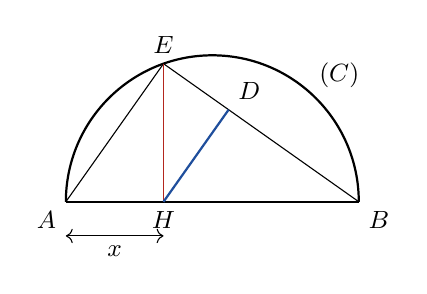
\begin{tikzpicture}[scale=0.62,font=\small]
\draw[thick] (6,0) arc (0:180:3);
\draw[thick] (0,0)--(6,0);
\coordinate (A) at (0,0); \coordinate (B) at (6,0); \coordinate (H) at (2,0);
\coordinate (E) at (2,2.828);
\draw (A)--(E)--(B); \draw[cThm] (E)--(H);
\coordinate (D) at ($(B)!(H)!(E)$);
\draw[cDef,thick] (H)--(D);
\node[below left] at (A){$A$}; \node[below right] at (B){$B$}; \node[below] at (H){$H$};
\node[above] at (E){$E$}; \node[above right] at (D){$D$};
\draw[<->] (0,-0.7)--(2,-0.7) node[midway,below]{$x$};
\node at (5.6,2.6){$(C)$};
\end{tikzpicture}
\end{LTR}\end{center}}
\end{tamrin}

% ------------------------------------------------- 20
\begin{tamrin}{أقصر مماس داخل مربع}
$ABCD$ مربع طول ضلعه $AB=2$. \ لتكن $(\Gamma)$ الدائرة التي مركزها $D$ ونصف قطرها $2$ ، و $M$ نقطة من القوس $\overset{\frown}{AC}$ تختلف عن $A$ و $C$. \ المماس $(T)$ للدائرة $(\Gamma)$ عند $M$ يقطع القطعة $[AB]$ في $K$ والقطعة $[BC]$ في $L$.\par
نريد تعيين وضعية $M$ حتى يأخذ الطول $KL$ أصغر قيمة ممكنة. نضع: $KB=x$ و $LB=y$.
\RL{0.6}{%
\textbf{1.} أثبت أن $KL^2=x^2+y^2$.\par
\textbf{2.} علماً أن $KA=KM$ و $LC=LM$ (مماسان من نقطة واحدة) ، أثبت أن $KL=4-x-y$ ، ثم استنتج أن:\\ $x^2+y^2=x^2+y^2-8x-8y+2xy+16$.\par
\textbf{3.} استنتج أن $y=\dfrac{4x-8}{x-4}$ ، ثم أن: $KL=\dfrac{-x^2+4x-8}{x-4}$.\par
\textbf{4.} لتكن $f$ الدالة المعرفة على $[0;2]$ بـ: $f(x)=\dfrac{-x^2+4x-8}{x-4}$. \ ادرس تغيرات $f$ ، واستنتج أن الطول $KL$ يأخذ أصغر قيمة ممكنة من أجل $x=4-2\sqrt2$.\par
\textbf{5.} عيّن عندئذ وضعية $M$.\par}
{0.37}{%
\begin{center}\begin{LTR}
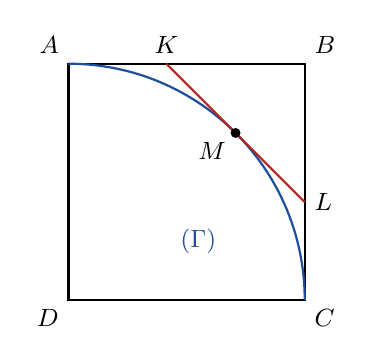
\begin{tikzpicture}[scale=1.5,font=\small]
\draw[thick] (0,0) rectangle (2,2);
\draw[cDef,thick] (2,0) arc (0:90:2);
\coordinate (D) at (0,0); \coordinate (A) at (0,2); \coordinate (B) at (2,2); \coordinate (C) at (2,0);
\coordinate (M) at (1.414,1.414);
\coordinate (K) at (0.828,2); \coordinate (L) at (2,0.828);
\draw[cThm,thick] (K)--(L);
\fill (M) circle(1.2pt);
\node[below left] at (D){$D$}; \node[above left] at (A){$A$}; \node[above right] at (B){$B$}; \node[below right] at (C){$C$};
\node[above] at (K){$K$}; \node[right] at (L){$L$}; \node[below left] at (M){$M$};
\node[cDef] at (1.1,0.5){$(\Gamma)$};
\end{tikzpicture}
\end{LTR}\end{center}}
\end{tamrin}

% ------------------------------------------------- 21
\begin{tamrin}{علبة بأكبر حجم}
لدينا قطعة من الورق المقوى مربعة الشكل طول ضلعها $12\ \text{cm}$. نقطع من أركانها الأربعة مربعات متقايسة طول ضلع كل منها $x$ (بالسنتيمتر) ، ثم نطوي الحواف لنحصل على علبة دون غطاء على شكل متوازي مستطيلات.
\begin{enumerate}
\item ما هي القيم الممكنة لـ $x$؟
\item بيّن أن حجم العلبة هو: $V(x)=x(12-2x)^2$.
\item ادرس تغيرات الدالة $V$ على المجال $]0;6[$.
\item استنتج قيمة $x$ التي يكون من أجلها حجم العلبة أكبر ما يمكن ، واحسب هذا الحجم.
\end{enumerate}
\end{tamrin}

% ------------------------------------------------- 22
\begin{tamrin}{المقارنة والمتباينات بواسطة المشتقة}
\begin{enumerate}
\item نعتبر العددين:
\[A=\frac{(5{,}012013014015016)^2+3}{3{,}012013014015016}\qquad\text{\ar{و}}\qquad B=\frac{(5{,}012013014015017)^2+3}{3{,}012013014015017}.\]
باستعمال الدالة $f:x\mapsto\dfrac{x^2+3}{x-2}$ ، قارن بين $A$ و $B$.
\item باستعمال دراسة دالة مناسبة ، بيّن أنه:
\begin{sq}
\qa من أجل كل عدد حقيقي $x\ge0$: $\sin x\le x$.
\qb من أجل كل عدد حقيقي $x\ge0$: $\sqrt{1+x}\le1+\dfrac x2$.
\end{sq}
\end{enumerate}
\end{tamrin}

\end{document}
